\hypersetup{
    bookmarks=true,         % show bookmarks bar?
    unicode=false,          % non-Latin characters in Acrobat’s bookmarks
    pdftoolbar=true,        % show Acrobat’s toolbar?
    pdfmenubar=true,        % show Acrobat’s menu?
    pdffitwindow=false,     % window fit to page when opened
    pdfstartview={FitH},    % fits the width of the page to the window
    pdftitle={My title},    % title
    pdfauthor={Author},     % author
    pdfsubject={Subject},   % subject of the document
    pdfcreator={Creator},   % creator of the document
    pdfproducer={Producer}, % producer of the document
    pdfkeywords={keyword1} {key2} {key3}, % list of keywords
    pdfnewwindow=true,      % links in new window
    colorlinks=false,       % false: boxed links; true: colored links
    linkcolor=red,          % color of internal links (change box color with linkbordercolor)
    citecolor=green,        % color of links to bibliography
    filecolor=magenta,      % color of file links
    urlcolor=cyan           % color of external links
}

\chapter{Benchmarks}
Below follows three benchmarks of different code sizes. All three benchmarks 
originate from the same code base, but the first is bench is on a code 10 times
the origin code, the second is 100 times the origin and the third is 1000 times
the origin. The code given as a string kept in the memory, that is the code is
not read from a file.

These test are done a system with the following specification:
\begin{center}
\begin{tabular}{l l}
Thing & Spec
\end{tabular}
\end{center}
There are benchmarks done on other systems as well and they follow the same trend.

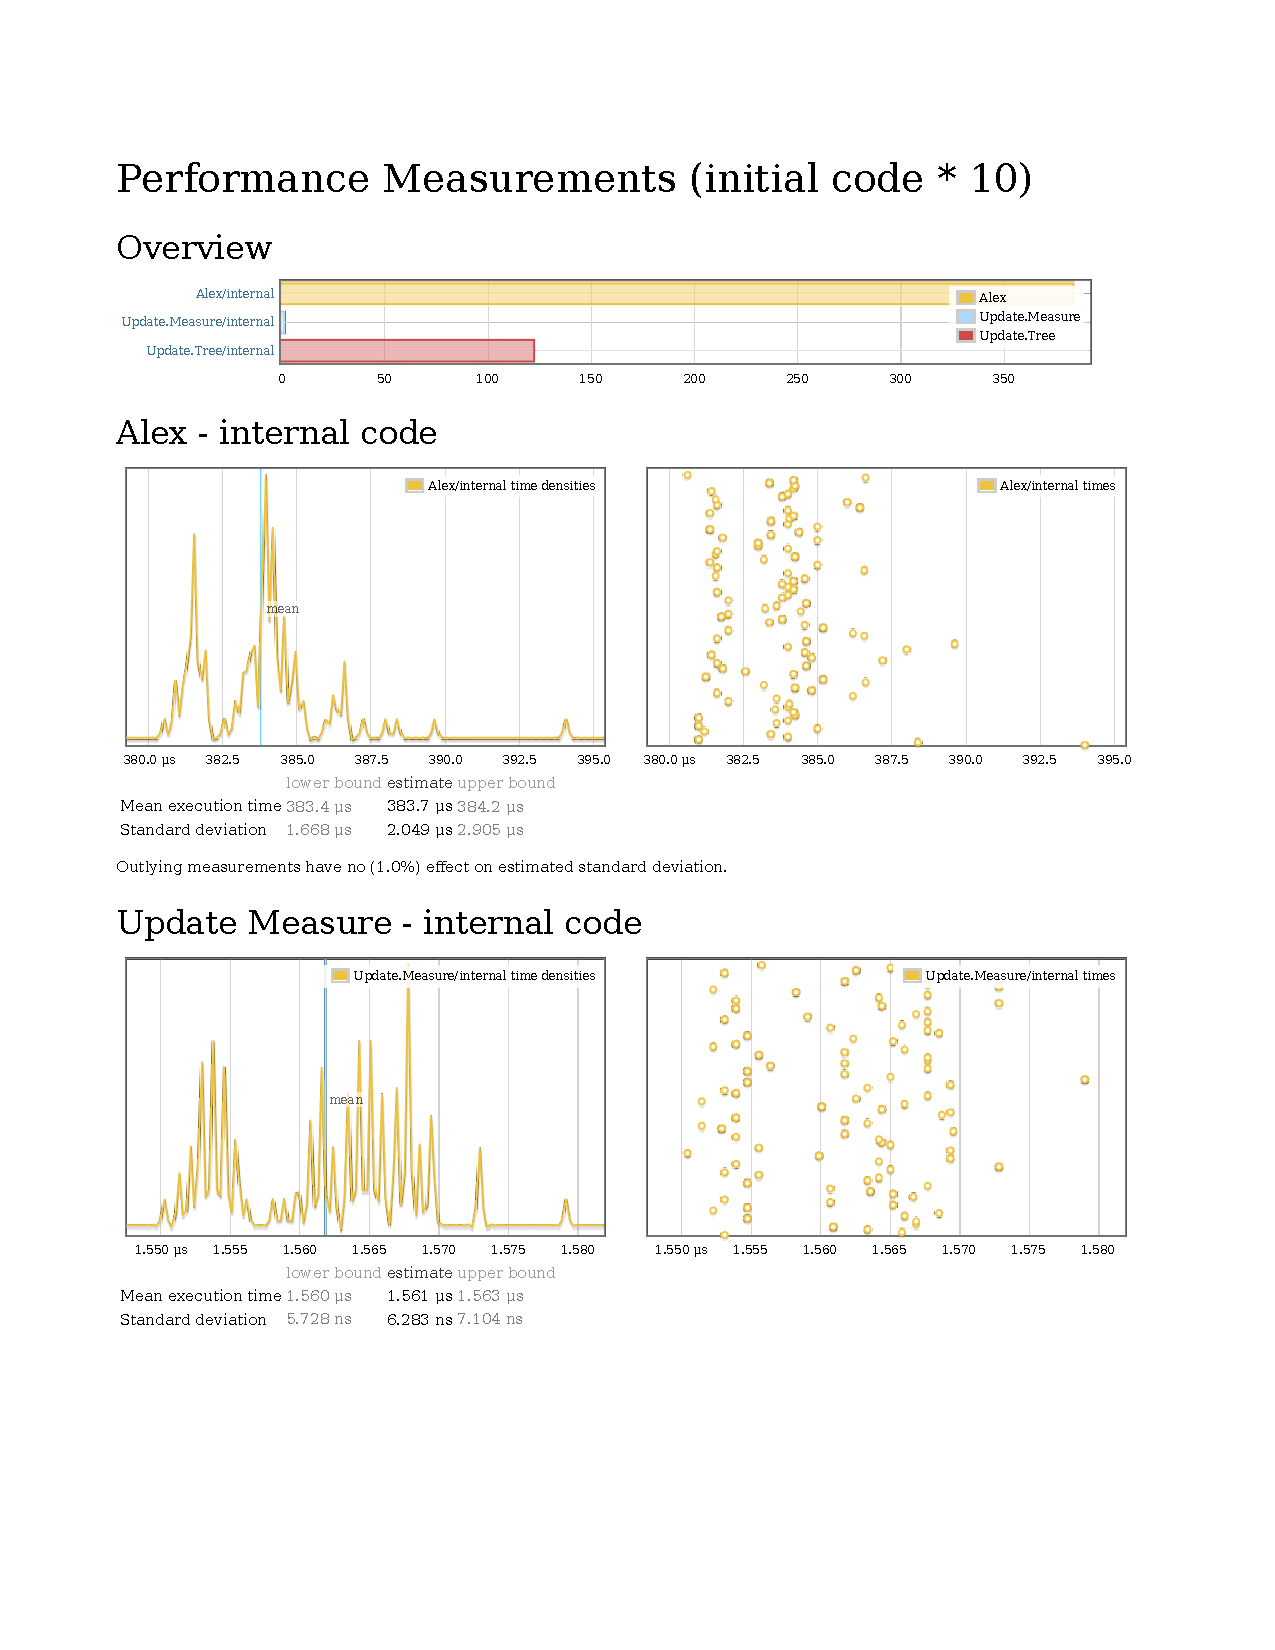
\includepdf[pages={1-2}]{tests/timepreformancebench10.pdf}
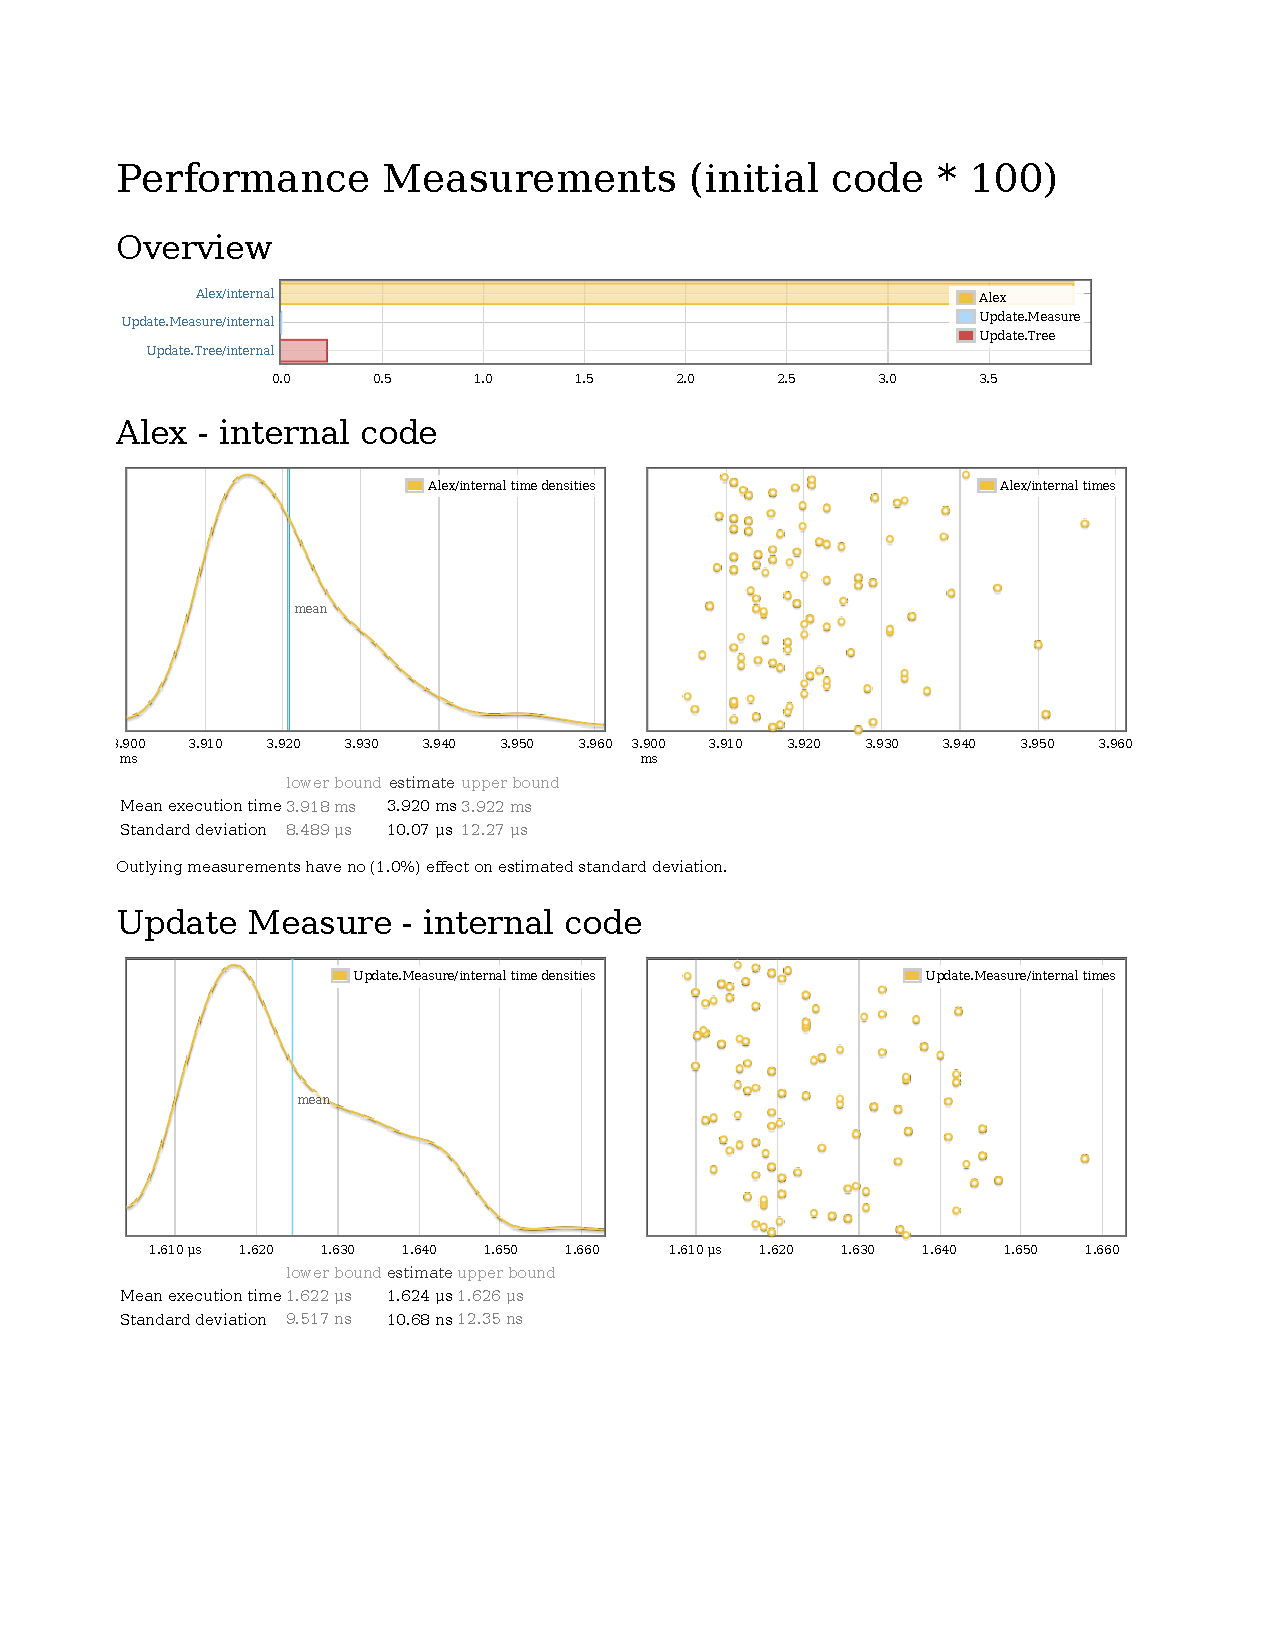
\includepdf[pages={1-2}]{tests/timepreformancebench100.pdf}
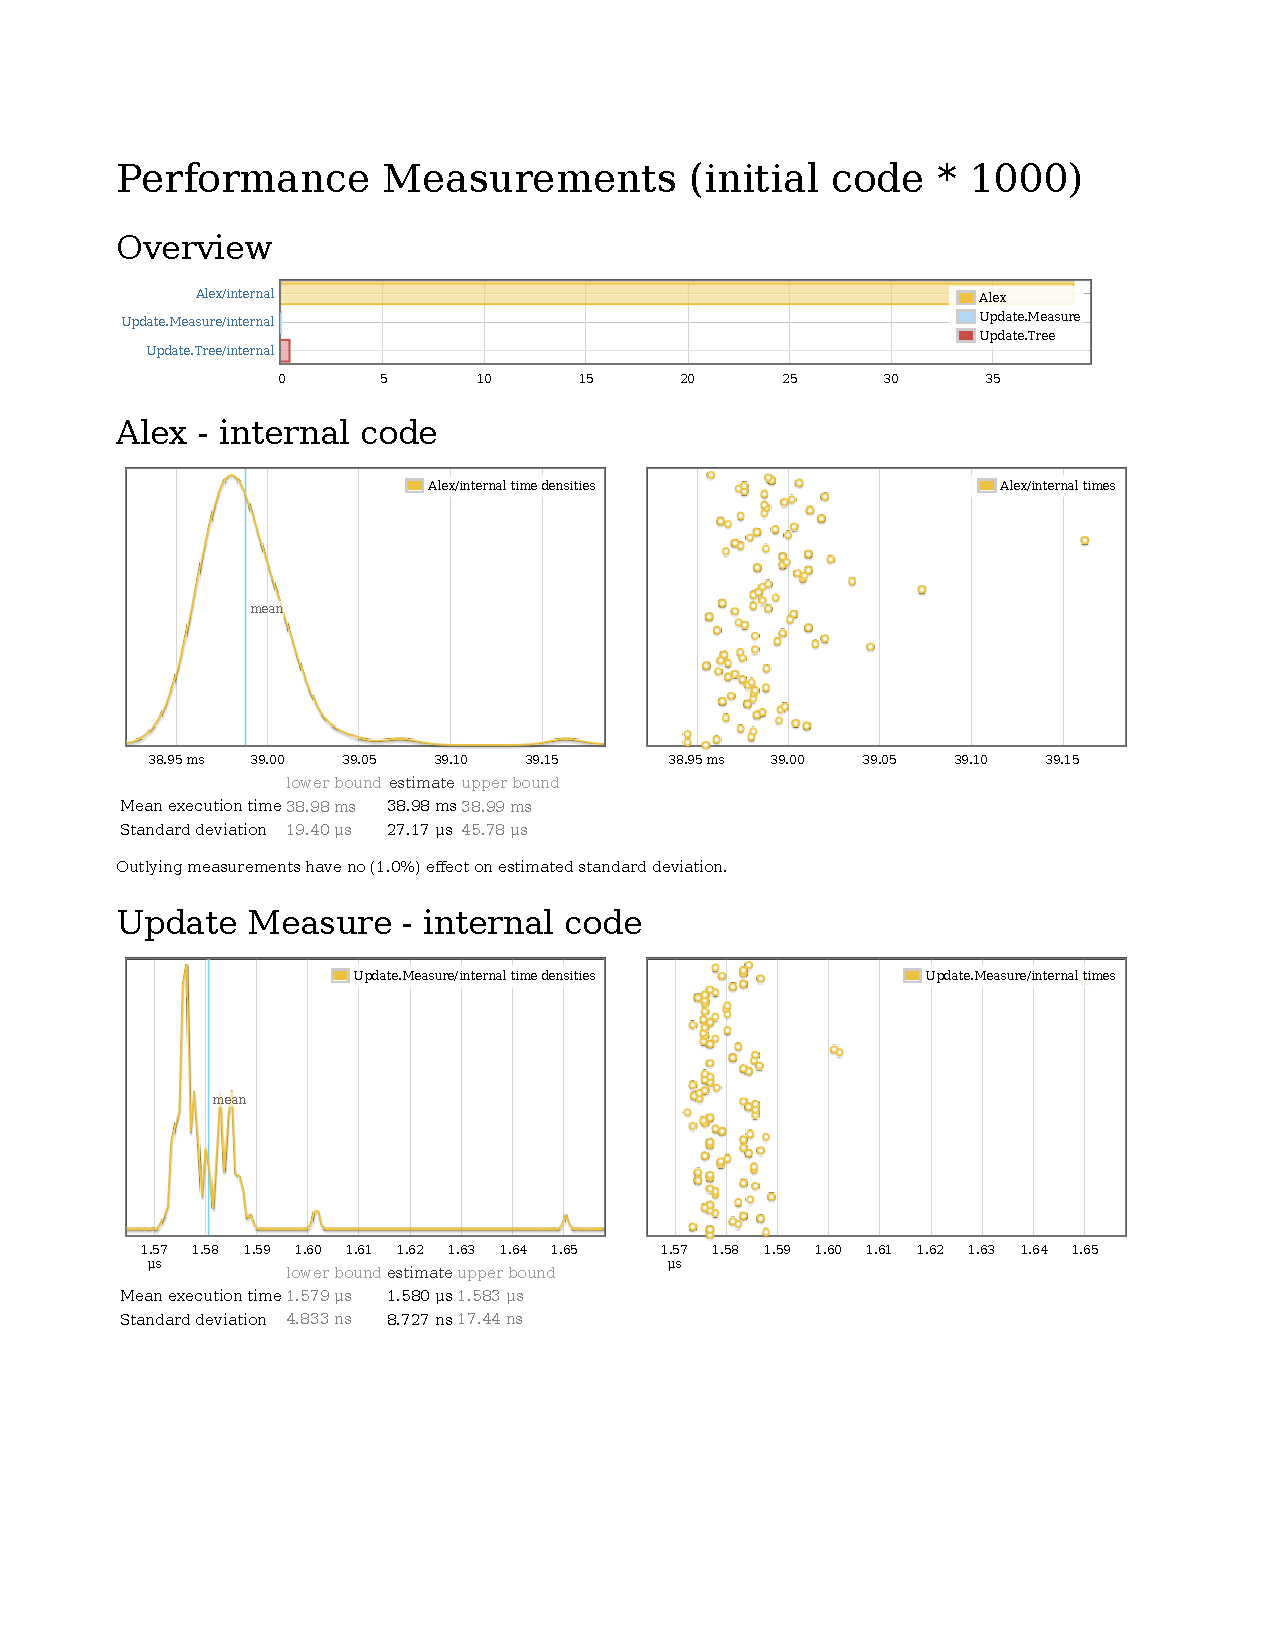
\includepdf[pages={1-2}]{tests/timepreformancebench1000.pdf}

\section*{Understanding the Graphs}
In this report, each function benchmarked by criterion is assigned
a section of its own.  In each section, we display two charts, each
with an $x$ axis that represents measured execution time.
These charts are active; if you hover your mouse over data points
and annotations, you will see more details.

\begin{itemize}
\item The chart on the left is a \href{http://en.wikipedia.org/wiki/Kernel_density_estimation}{kernel
    density estimate} (also known as a KDE) of time
    measurements. This graphs the probability of any given time
    measurement occurring. A spike indicates that a measurement of a
    particular time occurred; its height indicates how often that
    measurement was repeated.
\item The chart on the right is the raw data from which the kernel
    density estimate is built.  Measurements are displayed on
    the $y$ axis in the order in which they occurred.
\end{itemize}
   
Under the charts is a small table displaying the mean and standard
deviation of the measurements.  We use a statistical technique
called
the 
\href{http://en.wikipedia.org/wiki/Bootstrapping_(statistics)}{bootstrap}
to provide confidence intervals on our estimates of these values.
The bootstrap-derived upper and lower bounds on the mean and
standard deviation let you see how accurate we believe those
estimates to be. (Hover the mouse over the table headers to see
the confidence levels.)
   
A noisy benchmarking environment can cause some or many
measurements to fall far from the mean. These outlying
measurements can have a significant inflationary effect on the
estimate of the standard deviation. We calculate and display an
estimate of the extent to which the standard deviation has been
inflated by outliers.

These reports were created using the
\href{http://hackage.haskell.org/package/criterion}{criterion}
benchmark execution and performance analysis tool.
Criterion is developed and maintained
by \href{http://www.serpentine.com/blog/}{Bryan O'Sullivan}
